\documentclass[lang=zh]{sjtuarticle}	% Switch to lang=en for English
% !TEX root = ./main.tex

% rotate text
\usepackage{lscape}

% Chemistry formulae support
\usepackage[version=4]{mhchem}

% Circuit drawing support
\usepackage{circuitikz}
% Add arrows for transistors
\ctikzset{tripoles/mos style=arrows}
\ctikzset{transistors/arrow pos=end}
% \coord: Show the position of nodes
\def\normalcoord(#1){coordinate(#1)}
\def\showcoord(#1){coordinate(#1) node[
			circle, red, draw, inner sep=1pt, pin={[red, overlay, inner sep=0.5pt, font=\tiny, pin distance=0.1cm, pin edge={red, overlay}]45:#1}](){}}
\let\coord=\normalcoord
\let\coord=\showcoord % Comment this line to hide coordinates

% 使用 BibLaTeX 处理参考文献
%   biblatex-gb7714-2015 常用选项
%     gbnamefmt=lowercase     姓名大小写由输入信息确定
%     gbpub=false             禁用出版信息缺失处理
\usepackage[backend=biber,style=gb7714-2015]{biblatex}
% 文献表字体
% \renewcommand{\bibfont}{\zihao{5}\fixedlineskip{15.6bp}}
% 文献表条目间的间距
\setlength{\bibitemsep}{0pt}
% 导入参考文献数据库
\addbibresource{refs.bib}

% 脚注格式
\usepackage[perpage,bottom,hang]{footmisc}

% 定义图片文件目录与扩展名
\graphicspath{{figures/}}
\DeclareGraphicsExtensions{.pdf,.eps,.png,.jpg,.jpeg}

% 确定浮动对象的位置,可以使用 [H],强制将浮动对象放到这里(可能效果很差)
% \usepackage{float}

% 固定宽度的表格
% \usepackage{tabularx}

% 使用三线表:toprule,midrule,bottomrule。
\usepackage{booktabs}

% 表格中支持跨行
\usepackage{multirow}

% 表格中数字按小数点对齐
\usepackage{dcolumn}
\newcolumntype{d}[1]{D{.}{.}{#1}}

% 使用长表格
\usepackage{longtable}

% 附带脚注的表格
\usepackage{threeparttable}

% 附带脚注的长表格
\usepackage{threeparttablex}

% 算法环境宏包
\usepackage[ruled,vlined,linesnumbered]{algorithm2e}
% \usepackage{algorithm, algorithmicx, algpseudocode}

% 代码环境宏包
\usepackage{listings}
\lstdefinestyle{lstStyleCode}{%
  aboveskip         = \medskipamount,
  belowskip         = \medskipamount,
  basicstyle        = \ttfamily\zihao{6},
  commentstyle      = \slshape\color{black!60},
  stringstyle       = \color{green!40!black!100},
  keywordstyle      = \bfseries\color{blue!50!black},
  extendedchars     = false,
  upquote           = true,
  tabsize           = 2,
  showstringspaces  = false,
  xleftmargin       = 1em,
  xrightmargin      = 1em,
  breaklines        = false,
  framexleftmargin  = 1em,
  framexrightmargin = 1em,
  backgroundcolor   = \color{gray!10},
  columns           = flexible,
  keepspaces        = true,
  texcl             = true,
  mathescape        = true
}
\lstnewenvironment{codeblock}[1][]{%
  \lstset{style=lstStyleCode,#1}}{}

% 直立体数学符号
\providecommand{\dd}{\mathop{}\!\mathrm{d}}
\providecommand{\ee}{\mathrm{e}}
\providecommand{\ii}{\mathrm{i}}
\providecommand{\jj}{\mathrm{j}}

% 国际单位制宏包
\usepackage{siunitx}

% 定理环境宏包
\usepackage{ntheorem}
% \usepackage{amsthm}

% 绘图宏包
\usepackage{tikz}
\usetikzlibrary{arrows.meta, shapes.geometric}

% 数据图表宏包
\usepackage{pgfplots}
\pgfplotsset{compat=newest}

% 一些文档中用到的 logo
\usepackage{hologo}
\providecommand{\XeTeX}{\hologo{XeTeX}}
\providecommand{\BibLaTeX}{\textsc{Bib}\LaTeX}

% 借用 ltxdoc 里面的几个命令方便写文档
\DeclareRobustCommand\cs[1]{\texttt{\char`\\#1}}
\providecommand\pkg[1]{{\sffamily#1}}

% hyperref 宏包在最后调用
\usepackage{hyperref}

% E-mail
\providecommand{\email}[1]{\href{mailto:#1}{\urlstyle{tt}\nolinkurl{#1}}}


\begin{document}
\sloppy % Prevent overflowing lines due to hard-to-break entities

% !TEX root = ./report.tex

\begin{titlepage}
	\begin{center}
		
\includegraphics[width=\textwidth]{sjtu-vi-logo-red.pdf}
		\vspace*{1cm}

		\huge
		\textbf{本科课程项目报告} \\
		\Large
		\textbf{UNDERGRADUATE COURSE PROJECT REPORT}

		\vspace{2cm}
		\LARGE
		\textbf{基于 RISC-V 的处理器设计实现} \\

		\vfill

		\large
		\begin{minipage}{0.2\textwidth}
			\begin{flushleft}
				\Large
				姓\qquad 名: \\
				学\qquad 号: \\
				课\qquad 程: \\
				任课教师: \\
				学院(系) : \\
				开课学期: 
			\end{flushleft}
		\end{minipage}
		~
		\begin{minipage}{0.7\textwidth}
			\begin{center}
				\Large
				@ShabbyGayBar \\
				1145141919810 \\
				MST3305-通用及图形处理器架构与系统 \\
				景乃锋 \\
				电子信息与电气工程学院 \\
				2024年 (春季)
			\end{center}
		\end{minipage}
		
		%date
		\vspace{1cm}
		\Large
		\today
	\end{center}
\end{titlepage}

\tableofcontents
\newpage

\section{项目简介}

本项目实现了一个单周期以及一个5级流水线处理器。两种处理器均由 Verilog 语言编写,支持 RV32I Base Integer 指令集内的所有指令,包括:
\begin{codeblock}
add, sub, xor, or, and, sll, srl, sra, slt, sltu	// R-type
addi, xori, ori, andi, slli, srli, srai, slti, sltiu, lw, jalr	// I-type
sw	// S-type
beq, bne, blt, bge, bltu, bgeu	// B-type
lui, auipc	// U-type
jal	// J-type
\end{codeblock}

处理器顶层接口定义如表\ref{tab:top_io}所示。

\begin{table}[!htp]
	\centering
	\caption{处理器顶层接口定义}
	\label{tab:top_io}
	\begin{tabular}{|c|c|c|c|}
		\hline
		名称 & 输入/输出 & 说明  \\
		\hline
		clk & 输入 & 时钟信号 \\
		\hline
		rst & 输入 & 异步复位信号,高电平有效 \\
		\hline
		inst\_i & 输入 & 输入指令 \\
		\hline
		inst\_addr\_o & 输出 & 指令地址输出 \\
		\hline
		inst\_ce\_o & 输出 & 指令使能信号输出 \\
		\hline
		data\_i & 输入 & 读入的数据 \\
		\hline
		data\_we\_o & 输出 & 写使能控制信号 \\
		\hline
		data\_ce\_o & 输出 & 数据控制信号 \\
		\hline
		data\_addr\_o & 输出 & 读/写数据地址 \\
		\hline
		data\_o & 输出 & 写出的数据 \\
		\hline
	\end{tabular}
\end{table}

\section{设计流程}

\subsection{顶层模块}

流水线处理器的顶层模块划分如图\ref{fig:pipeline_stages}所示\cite{COD},其中指令和数据存储器作为外接设备,通过接口与处理器其他单元互动,本项目中不进行实现。

\begin{figure}[!htp]
	\centering
	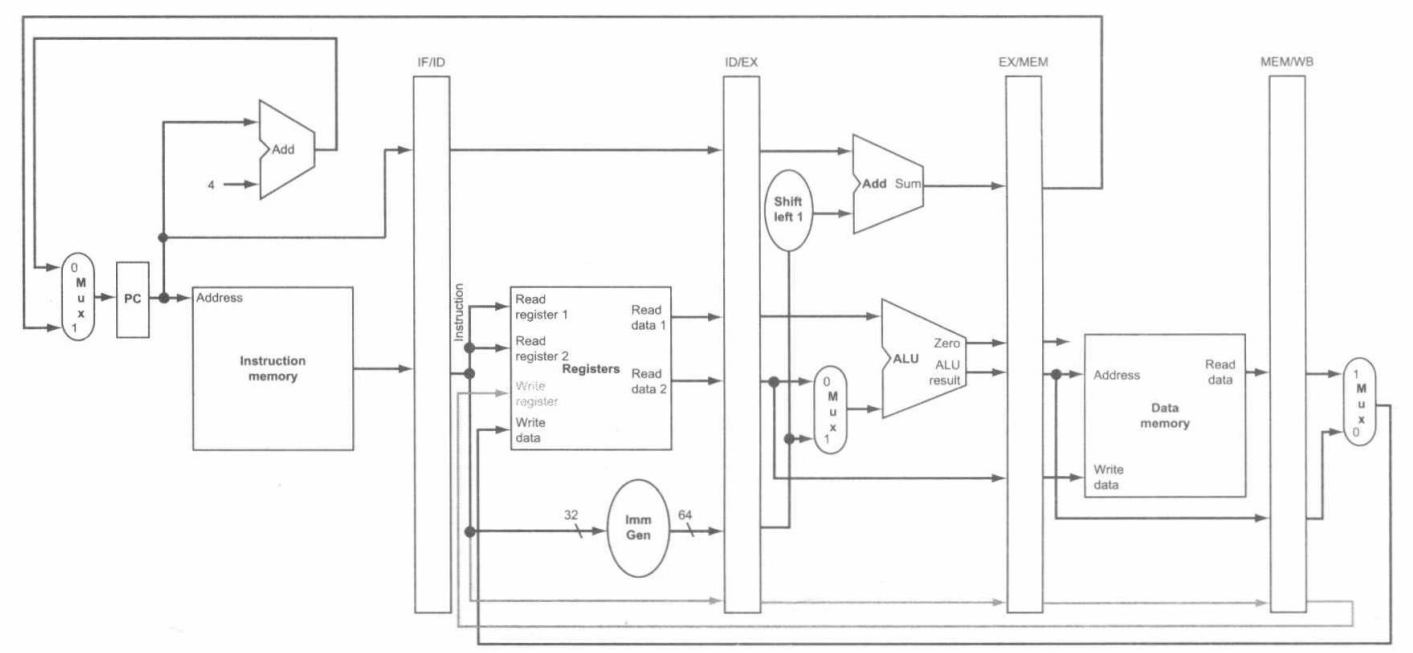
\includegraphics[width=\textwidth]{pipeline_stages.png}
	\caption{处理器顶层模块划分}
	\label{fig:pipeline_stages}
\end{figure}

在顶层设计中,每个流水段的组合逻辑被整合为一个模块。例如指令解码器和立即数生成器集成在 \texttt{riscv\_id.v} 中,ALU 和 EX 阶段的 PC 生成单元集成在 \texttt{riscv\_ex.v} 中。而寄存器被单独实现。这样的设计使得每个流水段模块可以独立测试,方便调试。

\subsection{单周期处理器}

单周期处理器作为流水线处理器的基础和蓝本,也有必要参照流水线处理器的设计思路进行模块划分,以便后续设计。与图\ref{fig:pipeline_stages}相比,单周期处理器不需要在相邻流水段之间插入寄存器,而是将所有组合逻辑之间直接相连。以下分别介绍每一流水段的设计思路和接口定义。

\subsubsection{指令读取模块}

指令读取 (Instruction Fetch, IF) 模块是单周期处理器中唯一需要时序控制的模块。其负责从指令存储器中读取指令,并将指令传递给下一个流水段。在单周期处理器中,指令读取模块的功能相对简单,只需实现程序计数器 (Program Counter, PC) 的自增、分支功能即可,当前指令由指令存储器接口 inst\_i 提供,无需由此模块输出。程序计数器作为指令存储器的地址输入,用于指示当前指令的地址。IF 模块接口定义如表\ref{tab:single_if_io}所示。

\begin{table}[!htp]
	\centering
	\caption{指令读取模块接口定义}
	\label{tab:single_if_io}
	\begin{tabular}{|c|c|c|c|}
		\hline
		名称 & 输入/输出 & 说明 & 来源/去向 \\
		\hline
		clk & 输入 & 时钟信号 & 外部 \\
		\hline
		rst & 输入 & 异步复位信号 & 外部 \\
		\hline
		br\_i & 输入 & 分支信号 & EX \\
		\hline
		pc\_i & 输入 & 下一程序计数器 & EX \\
		\hline
		pc\_o & 输出 & 当前程序计数器 & 指令存储器 \\
		\hline
	\end{tabular}
\end{table}

在每个时钟上升沿,程序计数器默认会自增4,即指向下一条指令。然而当分支信号 br\_i 为1时,程序计数器会跳转到 pc\_i 所指示的地址。异步复位信号 rst 为1时,程序计数器为0。

\subsubsection{指令译码模块}
\label{sec:single_id}

指令译码 (Instruction Decode, ID) 模块负责解析指令的操作码,识别指令类型,从指令中提取操作数,还包含了寄存器堆以供读写。另外,为了方便,本项目将图\ref{fig:pipeline_stages}中原属于执行 (EX) 模块的 ALU 输入部分的组合逻辑也整合进了译码器,使得 ID 模块的输出可直接提供给 ALU。ID 模块接口定义如表\ref{tab:single_id_io}所示。

\begin{table}[!htp]
	\centering
	\caption{指令译码模块接口定义}
	\label{tab:single_id_io}
	\begin{tabular}{|c|c|c|c|}
		\hline
		名称 & 输入/输出 & 说明 & 来源/去向 \\
		\hline
		inst\_i & 输入 & 当前指令 & 指令存储器 \\
		\hline
		rd\_val\_i & 输入 & 目的寄存器写入数据 & WB \\
		\hline
		rs2\_val\_o & 输出 & rs2 寄存器值,用于 S 型指令 & 数据存储器 \\
		\hline
		alu\_op\_o & 输出 & ALU 操作码 & EX \\
		\hline
		alu\_a\_o & 输出 & 第一个操作数,通常为 rs1 & EX \\
		\hline
		alu\_b\_o & 输出 & 第二个操作数 & EX \\
		\hline
		offset\_o & 输出 & B 型指令中的 PC 偏移量 & EX \\
		\hline
		br\_o & 输出 & 分支信号 & EX \\
		\hline
		zero\_en\_o & 输出 & 零标志位使能,用于分支判断 & EX \\
		\hline
		data\_we\_o & 输出 & 数据存储器写使能 & 数据存储器, WB \\
		\hline
		data\_re\_o & 输出 & 数据存储器读使能,同Mem2Reg\cite{COD} & WB \\
		\hline
	\end{tabular}
\end{table}

除了组合逻辑外,ID 模块还包含了一个寄存器堆,用于存储32个通用寄存器的值。寄存器堆的读操作为组合逻辑,由 ID 模块的 rs1\_idx\_i 和 rs2\_idx\_i 控制,输出 rs1 和 rs2 的实时值 rs1\_val\_o 和 rs2\_val\_o;写操作为时序逻辑,由 ID 模块解析当前指令得到的 rd\_we 控制,在每个时钟上升沿将 WB 模块的 rd\_val\_i 写入目的寄存器。

\subsubsection{执行模块}

执行 (Execute, EX) 模块负责执行指令,包括算术逻辑运算、移位运算、比较运算、分支跳转等。EX 模块接口定义如表\ref{tab:single_ex_io}所示。	

\begin{table}[!htp]
	\centering
	\caption{执行模块接口定义}
	\label{tab:single_ex_io}
	\begin{tabular}{|c|c|c|c|}
		\hline
		名称 & 输入/输出 & 说明 & 来源/去向 \\
		\hline
		pc\_i & 输入 & 当前程序计数器 & IF \\
		\hline
		alu\_op\_i & 输入 & ALU 操作码 & ID \\
		\hline
		alu\_a\_i & 输入 & 第一个操作数 & ID \\
		\hline
		alu\_b\_i & 输入 & 第二个操作数 & ID \\
		\hline
		zero\_en\_i & 输入 & 零标志位使能 & ID \\
		\hline
		br\_i & 输入 & 分支信号 & ID \\
		\hline
		offset\_i & 输入 & 分支跳转偏移量 & ID \\
		\hline
		br\_o & 输出 & 分支信号 & IF \\
		\hline
		pc\_o & 输出 & 下一程序计数器 & IF \\
		\hline
		data\_addr\_o & 输出 & 数据存储器地址 (即 ALU 运算结果) & 数据存储器 \\
		\hline
	\end{tabular}
\end{table}

EX 模块主要由两部分组成:ALU 和分支跳转。

ALU 根据操作码 alu\_op\_i 执行运算,将结果 data\_addr\_o 传递给数据存储器。

分支跳转组合逻辑则在 br\_i 为高 (即 ID 模块解析到 B 型指令) 时根据 ALU 的零标志位判断是否需要跳转地址,计算下一程序计数器 pc\_o 并将其与分支信号 br\_o 和输出给 IF 模块。

\subsubsection{写回模块}

写回 (Write Back, WB) 模块负责将执行模块的运算结果写回寄存器堆。WB 模块接口定义如表\ref{tab:single_wb_io}所示。

\begin{table}[!htp]
	\centering
	\caption{写回模块接口定义}
	\label{tab:single_wb_io}
	\begin{tabular}{|c|c|c|c|}
		\hline
		名称 & 输入/输出 & 说明 & 来源/去向 \\
		\hline
		data\_i & 输入 & 数据存储器读出数据 & 数据存储器 \\
		\hline
		data\_addr\_i & 输入 & 数据存储器地址 & EX \\
		\hline
		data\_re\_i & 输入 & 数据存储器读使能,同Mem2Reg\cite{COD} & ID \\
		\hline
		rd\_val\_o & 输出 & 目的寄存器写入数据 & ID (寄存器堆) \\
		\hline
	\end{tabular}
\end{table}

WB 模块实际上就是一个2输入1输出的多路选择器 (Multiplexer, MUX),根据 data\_re\_i 信号选择数据存储器读出的数据 data\_i 或者 EX 模块的运算结果 data\_addr\_i 作为目的寄存器写入数据 rd\_val\_o。

\subsubsection{Vivado 综合结果}

\subsection{流水线处理器}

流水线处理器的设计基于单周期处理器,将五个流水段:取指 (IF)、译码 (ID)、执行 (EX)、访存 (MEM)、写回 (WB) 的组合逻辑分离出来,每两段之间插入寄存器,并增加了停顿与前递等数据冒险处理逻辑,如图\ref{fig:pipeline_stages}所示。

组合逻辑只需要细微的改动,寄存器的实现逻辑也较简单,此处不再赘述。以下将介绍流水线处理器中的数据冒险处理逻辑。

\subsubsection{停顿}

停顿 (Stalling) 是一种数据冒险处理技术。当一个指令需要读取另一条指令尚未写回的结果时,流水线处理器会在执行阶段停顿一周期,等待数据准备好。需要使用停顿的情境通常有:

\begin{enumerate}
	\item 上一指令为 load 指令,当前的 ID 阶段却需要读取 load 指令的结果。 \\
	此时只需要暂停 IF 和 ID 阶段的指令传递即可,下一周期 ID 模块的译码器将通过前递逻辑直接读取数据存储器的结果。
	\item 分支信号激活,需要跳转到另一地址。 \\
	此时则应该通过清零 ID-EX 寄存器插入一个气泡,实现 ID 阶段的停顿。
	\item 指令或数据存储器由于读写冲突等原因暂时无法读写。 \\
	这种情况由于顶层模块以及指令、数据存储器并没有相应的接口,因此不予考虑。
\end{enumerate}

\subsubsection{前递}

前递 (Forwarding) 指将 EX 阶段的运算结果或 MEM 阶段的数据直接传递给 ID 阶段,是另一种数据冒险处理技术。需要前递的情境通常是当一个指令需要读取另一条指令尚未写回的结果时,因此本项目中,前递逻辑主要集中在执行阶段和译码阶段之间,以及访存阶段和译码阶段之间。

值得注意的是,教材\cite{COD}中,前递信号被传递给了 EX 模块中的多路选择器 (MUX),将其他流水段寄存器的值作为 ALU 的输入。然而在本项目中,如第\ref{sec:single_id}节所述,这部分组合逻辑被整合到了 ID 模块中,因此前递信号直接取代了 ID 模块的 rs1\_val\_id 和 rs2\_val\_id。原先寄存器堆的输出 rs1\_val\_o 和 rs2\_val\_o 作为前递控制逻辑的输入,在前递信号有效时,其值将被前递的数据覆盖。

\subsubsection{Vivado 综合结果}

\section{测试}

\subsection{代码例化层次}

本项目的测试 (Testbench) 的顶层代码为 \texttt{riscv\_soc\_tb.v},其中调用了处理器的顶层模块 \texttt{riscv.v},以及指令 (inst\_mem) 和数据存储器 (data\_mem),例化层次如图\ref{fig:hierarchy}所示。

\begin{figure}[!htp]
	\centering
	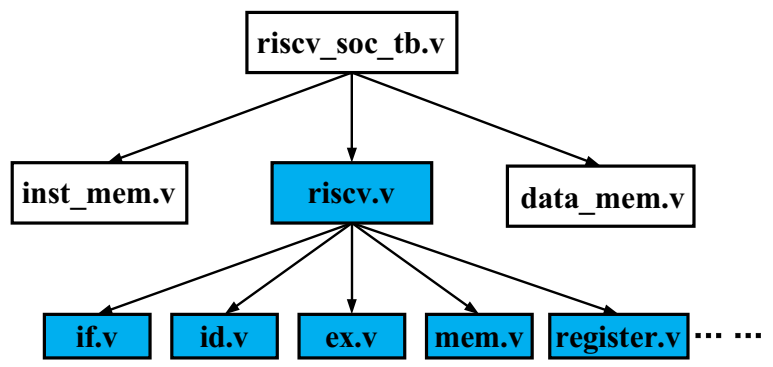
\includegraphics[scale=0.5]{hierarchy.png}
	\caption{处理器测试代码例化层次}
	\label{fig:hierarchy}
\end{figure}

其中,\texttt{riscv\_soc\_tb.v} 和存储器的接口与代码由课程组提供,不得更改,但是指令存储器和数据存储器的内容可以自行修改。

\subsection{测试程序}

考虑到课程提供的测试程序 (即指令存储器内容) 涵盖的指令和数据冒险情况较少,因此本项目选择参考 \href{https://github.com/cgyurgyik/riscv-assembly/blob/master/quicksort.s}{cgyurgyik 的快速排序 RISC-V 汇编程序}作为测试程序。该程序将一个数组 (10, 80, 30, 90, 40, 50, 70) 从小到大排序,排序结果为 (10, 30, 40, 50, 70, 80, 90) 并存储在数据存储器的地址 0x0000-0x001b 处。

在此基础上,本项目稍作修改,将排序好的数组写入寄存器 x10-x16,以便在 GTKWave 中查看排序结果。

\subsection{仿真流程}

由于 cgyurgyik 的程序是由 RISC-V 汇编语言编写的,需要转换成指令存储器中的 32 位二进制指令。而课程组提供的转换程序不支持部分 RV32I 指令集指令,如 slli,因此本项目采用 \href{https://github.com/Kritagya-Agarwal/Assembly-To-Machine-Code-RISC-V}{Kritagya Agarwal 的 \textit{Assembly To Machine Code Translation} 工具}进行转换。

最后,本项目使用 \href{https://github.com/steveicarus/iverilog}{Icarus Verilog 仿真器}进行仿真,通过 \href{https://github.com/gtkwave/gtkwave}{GTKWave} 查看波形图,验证设计的正确性。

\subsection{结果分析}

单周期处理器和流水线处理器运行测试程序的仿真结果分别如图\ref{fig:wave_single}和图\ref{fig:wave_pipeline}所示。

\begin{figure}[!htp]
	\centering
	\begin{minipage}{\textwidth}
		\centering
		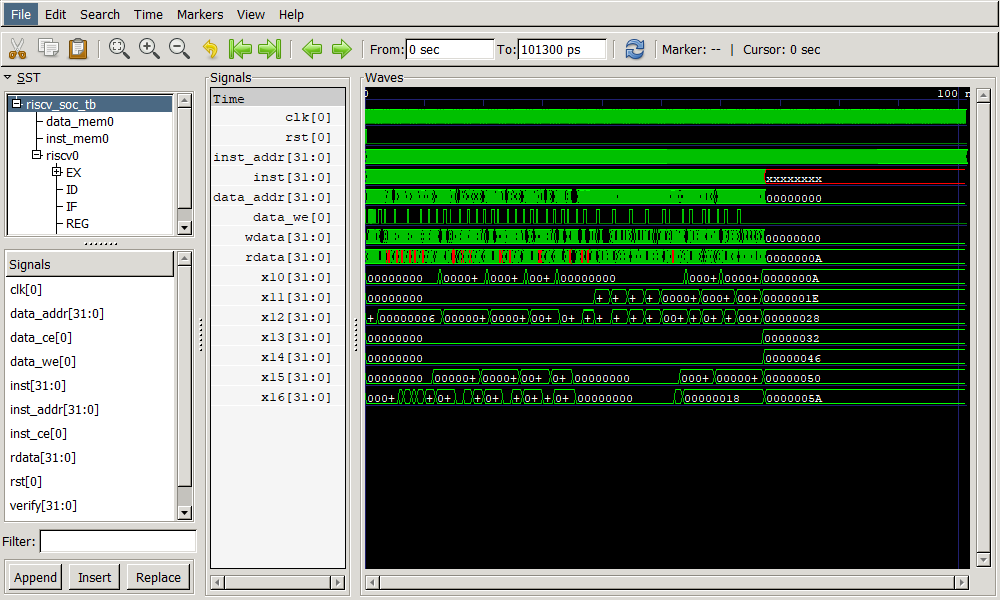
\includegraphics[width=\textwidth]{wave_single.png}
		\caption{单周期处理器波形图}
		\label{fig:wave_single}
	\end{minipage}
	\begin{minipage}{\textwidth}
		\centering
		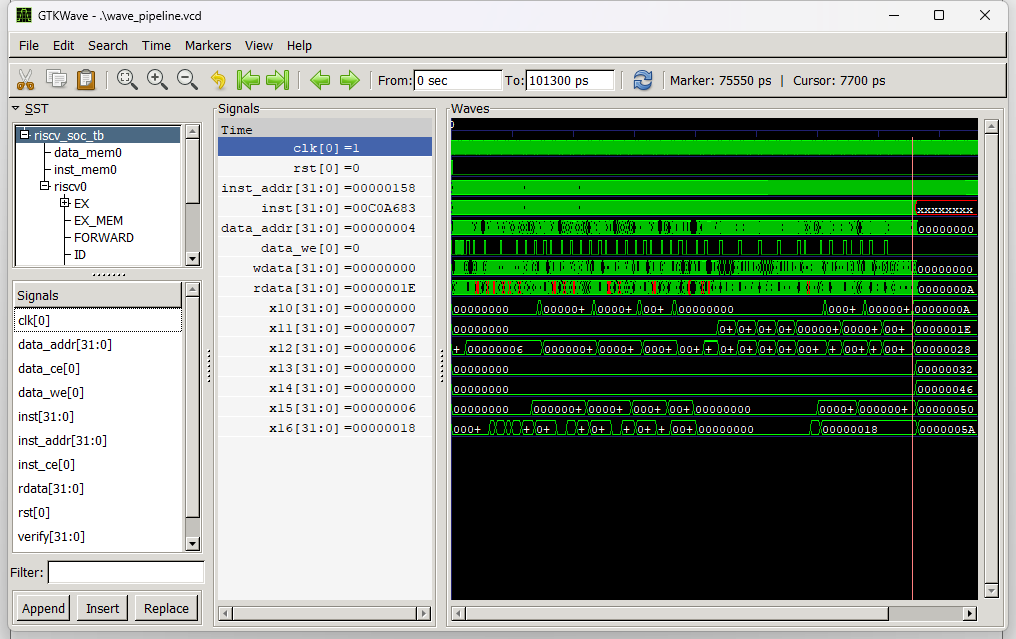
\includegraphics[width=\textwidth]{wave_pipeline.png}
		\caption{流水线处理器波形图}
		\label{fig:wave_pipeline}
	\end{minipage}
\end{figure}

从波形图中可以看出,x10-x16寄存器最后的值都是排好序的数组,说明单周期处理器和流水线处理器均能正确执行快速排序的测试程序。

放大波形图\ref{fig:wave_pipeline}至\SI{19.30}{\ns}附近,如图\ref{fig:pipeline_stall}所示,此时流水线正在执行如下指令:

\begin{codeblock}
0x0008AF03	// lw x30, 0(x17)
0x01E82023	// sw x30, 0(x16)
0x01C8A023	// sw x28, 0(x17)
0x00138393	// addi x7, x7, 1
0xFC0006E3	// beq x0, x0, LOOP
//0x00130F13	// addi x30, x6, 1, NOT EXECUTED DUE TO STALL SIGNAL
0x02C38C63	// beq x7, x12, LOOP_DONE
\end{codeblock}

\begin{figure}[!htp]
	\centering
	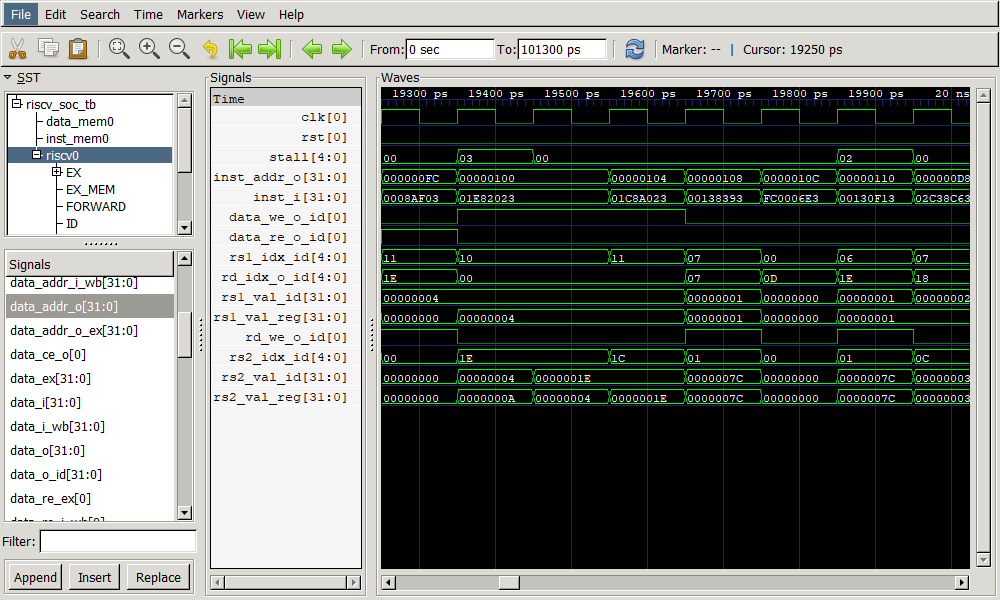
\includegraphics[width=\textwidth]{wave_pipeline_stall.png}
	\caption{流水线处理器停顿示意图}
	\label{fig:pipeline_stall}
\end{figure}

根据图\ref{fig:pipeline_stall}可以发现,当执行第2条 sw 指令时,前一条 lw 指令的结果还未读取,因此流水线处理器不得不产生 stall 信号,在此处停顿一周期,等待数据读取至 MEM 流水段的 data\_i 中,并通过前递逻辑传递给 ID 流水段,从而继续执行 sw 指令。在波形图中体现为 0x01E82023 指令在 stall 信号变为 0x0011 后多占用了一个周期。

而当执行第5条 beq 指令时,由于是否跳转的判断需要在 EX 阶段,即下下个周期才能得出,因此流水线处理器在此处产生 0x0010 的 stall 信号,停顿一周期,等待判断结果。但是此时下一条指令 (addi x30, x6, 1) 已经由 IF 流水段读取,因此需要在此指令的 ID 阶段插入一个气泡,将 ID-EX 寄存器清零,使其成为 nop,实现停顿。

对比两波形图可以发现,在\SI{10}{\GHz}时钟频率下,单周期处理器完成测试程序执行所需的时间为\SI{66.75}{\ns},而流水线处理器执行完成所需的时间为\SI{75.50}{\ns},流水线处理器的执行时间比单周期处理器更长,这似乎与流水线处理器的指令吞吐量更高的设计初衷相悖。然而,这是因为流水线处理器由于每个时钟周期内的延迟更少,可以有更高的时钟频率,而测试中这一优势并未体现,而且由于流水线处理器存在数据冒险的情况,需要停顿,因此导致流水线处理器的执行时间更长。假设流水线处理器的时钟频率提高到\SI{50}{\GHz},则流水线处理器的执行时间会压缩到\SI{15.10}{\ns},大大快于单周期处理器。

\section{总结}

本项目实现了一个单周期处理器和一个5级流水线处理器,支持 RV32I Base Integer 指令集内的所有指令。通过仿真测试,验证了两种处理器的功能正确性。流水线处理器的设计使得其在时钟频率更高的情况下能够有更高的性能,但是由于数据冒险的存在,可能导致流水线处理器的延迟更长。

本项目已发表至 \href{https://github.com/ShabbyGayBar/RISCV_CPU}{GitHub}。

\nocite{*}
\printbibliography

\end{document}
